%-----------------------------------------------------------------------
% Beginning of chap2.tex
%-----------------------------------------------------------------------
%
%  AMS-LaTeX sample file for a chapter of a monograph, to be used with
%  an AMS monograph document class.  This is a data file input by
%  chapter.tex.
%
%  Use this file as a model for a chapter; DO NOT START BY removing its
%  contents and filling in your own text.
% 
%%%%%%%%%%%%%%%%%%%%%%%%%%%%%%%%%%%%%%%%%%%%%%%%%%%%%%%%%%%%%%%%%%%%%%%%


\chapter*{Lecture 13}
\addcontentsline{toc}{chapter}{Lecture 12}
\addtocounter{chapter}{3}
\addtocounter{section}{0}
%\numberwithin{section}{chapter}
\numberwithin{equation}{chapter}
\numberwithin{theorem}{chapter}

%\epigraph{}{--- \textup{}}

Primal-dual interior point methods aim to solve the problem
\begin{equation}\label{eq:standard}\tag{P}
 \minimize \ip{\vct{c}}{\vct{x}} \quad \subjto \mtx{A}\vct{x}=\vct{b}, \ \vct{x}\geq \zerovct
\end{equation}
for a matrix $\mtx{A}\in \R^{m\times d}, \vct{b}\in \R^m$ and $\vct{c}\in \R^d$, by applying Newton-type iterations to the optimality conditions of linear programming. More precisely, we have seen the following algorithm. Recall the feasible sets
\begin{align*}
 \mathcal{F} &= \{(\vct{y},\vct{s},\vct{x}) \mid \mtx{A}^{\trans}\vct{y}+\vct{s}=\vct{c}, \ \mtx{A}\vct{x}=\vct{b}, \ \vct{x}\geq \zerovct, \ \vct{s}\geq \zerovct\}\\
 \mathcal{F}^{\circ} &= \{(\vct{y},\vct{s},\vct{x}) \mid \mtx{A}^{\trans}\vct{y}+\vct{s}=\vct{c}, \ \mtx{A}\vct{x}=\vct{b}, \ \vct{x}> \zerovct, \ \vct{s}> \zerovct\}\\
\end{align*}
The a simple primal-dual interior point method can be described as follows.
\begin{itemize}
 \item Start with $(\vct{x}^{(0)},\vct{y}^{(0)},\vct{s}^{(0)})\in \mathcal{F}^{\circ}$;
 \item For each $k\geq 0$, compute the duality parameter
 \begin{equation*}
  \mu^{(k)} = \frac{1}{d} \sum_{i=1}^d x_is_i
 \end{equation*}
and choose $\sigma_k\in [\sigma_{\mathrm{min}},\sigma_{\mathrm{max}}]$. Solve
\begin{equation*}
 \begin{pmatrix}
  \zerovct & \mtx{A}^{\trans} & \mtx{I} \\
  \mtx{A} & \zerovct & \zerovct \\
  \mtx{S}^{(k)} & \zerovct & \mtx{X}^{(k)}
 \end{pmatrix}
\begin{pmatrix} \Delta\vct{x}\\ \Delta \vct{y}\\ \Delta\vct{s} \end{pmatrix} = \begin{pmatrix} \zerovct \\ \zerovct \\ -\vct{X}^{(k)}\mtx{S}^{(k)}\vct{e}+\sigma \mu^{(k)}\end{pmatrix}
\end{equation*}
and compute
\begin{equation*}
\begin{pmatrix} \vct{x}^{k+1}\\ \vct{y}^{k+1}\\ \vct{s}^{k+1}\end{pmatrix}= \begin{pmatrix} \vct{x}^{k}\\ \vct{y}^{k}\\ \vct{s}^{k}\end{pmatrix} +\alpha_k \begin{pmatrix} \Delta\vct{x}\\ \Delta \vct{y}\\ \Delta\vct{s} \end{pmatrix},
 \end{equation*}
for a small enough $\alpha_k>0$ to ensure non-negativity.
\end{itemize}

In each iteration, a Newton step is taken in the direction of the {\em central path}. This is a curve in $\mathcal{F}^{\circ}$ defined as the set of solutions of
\begin{align}\label{eq:cpopt}
 \begin{split}
  \mtx{A}^{\trans}\vct{y}+\vct{s}-\vct{c} &= \zerovct\\
  \mtx{A}\vct{x}-\vct{b} & = \zerovct\\
  \mtx{X}\mtx{S}\vct{e} &= \tau \vct{e}\\
  \vct{x}&> \zerovct\\
  \vct{s}&> \zerovct,
 \end{split}
\end{align}
where $\tau>0$. 

\section{Path-following methods}
A path-following method tries to ensure that each iterate is {\em close} to the central path. What it means to be close to the central path depends on the neighbourhood we choose. Here, we will look at the (one-sided) $\infty$-norm neighbourhood
\begin{equation*}
\mathcal{N}_{-\infty}(\gamma) = \{(\vct{x},\vct{y},\vct{s})\in \mathcal{F}^{\circ} \mid x_is_i\geq \gamma \mu, \ 1\leq i\leq d\}
\end{equation*}
for some $\gamma\in (0,1]$ (say, $\gamma=10^{-3}$). In words, each $x_is_i$ has to be at least some small multiple of their average value. To see what this has to do with the $\infty$-norm neighbourhood, consider the set of $\vct{x}$ such that
\begin{equation*}
 \norm{\mtx{X}\mtx{S}\vct{e}-\mu \vct{e}}_\infty \leq (1-\gamma) \mu \ \Longleftrightarrow \ \forall 1\leq i\leq d, \ \gamma \mu \leq x_is_i \leq 2-\gamma,
\end{equation*}
and we are only interested in the lower inequality.

The so-called {\em long-step path-following} interior point method can then be described as follows.
\begin{itemize}
 \item Start with $(\vct{x}^{(0)},\vct{y}^{(0)},\vct{s}^{(0)})\in \mathcal{N}_{-\infty}(\gamma)$;
 \item For each $k\geq 0$, compute the duality parameter
 \begin{equation*}
  \mu^{(k)} = \frac{1}{d} \sum_{i=1}^d x_is_i
 \end{equation*}
and choose $\sigma_k\in [\sigma_{\mathrm{min}},\sigma_{\mathrm{max}}]$. Solve
\begin{equation*}
 \begin{pmatrix}
  \zerovct & \mtx{A}^{\trans} & \mtx{I} \\
  \mtx{A} & \zerovct & \zerovct \\
  \mtx{S}^{(k)} & \zerovct & \mtx{X}^{(k)}
 \end{pmatrix}
\begin{pmatrix} \Delta\vct{x}\\ \Delta \vct{y}\\ \Delta\vct{s} \end{pmatrix} = \begin{pmatrix} \zerovct \\ \zerovct \\ -\vct{X}^{(k)}\mtx{S}^{(k)}\vct{e}+\sigma \mu^{(k)}\end{pmatrix}
\end{equation*}
and compute
\begin{equation*}
\begin{pmatrix} \vct{x}^{k+1}\\ \vct{y}^{k+1}\\ \vct{s}^{k+1}\end{pmatrix}= \begin{pmatrix} \vct{x}^{k}\\ \vct{y}^{k}\\ \vct{s}^{k}\end{pmatrix} +\alpha_k \begin{pmatrix} \Delta\vct{x}\\ \Delta \vct{y}\\ \Delta\vct{s} \end{pmatrix},
 \end{equation*}
for a small enough $\alpha_k\in [0,1]$ is the largest value such that $(\vct{x}^{(k+1)},\vct{y}^{(k+1)},\vct{s}^{(k+1)})\in \mathcal{N}_{-\infty}(\gamma)$.
\end{itemize}

\begin{remark}
 As noted at the end of Lecture 11, to find an initial point in $\mathcal{F}^{\circ}$ might not be trivial. In practice one can therefore also use the algorithm described above using {\em infeasible} points, though in this case we have to make sure that the residual norms $\norm{\vct{b}-\mtx{A}\vct{x}}$ and $\norm{\vct{c}-\vct{s}-\mtx{A}^{\trans}\vct{y}}$ remain bounded.
\end{remark}

\subsection{Visualising the algorithm}
The feasible set $\mathcal{F}^{\circ}$ usually lives in a space that can't be easily visualised, but if the dual version is two-dimensional,
\begin{equation*}
 \{\vct{y}\in \R^2 \mid \mtx{A}^{\trans}\vct{y}+\vct{s}=\vct{c}, \ \vct{s}\geq \zerovct\},
\end{equation*}
then we have a chance to see how the trajectories of the iterates in $\vct{y}$ look like.
Consider, for example, the linear programming problem whose dual is given by
\begin{align*}
\maximize & y_1+y_2\\
\subjto & 0.2py_1+y_2+s_p = 1+0.01p^2, \ 0\leq p\leq 10.
\end{align*}
The points $\vct{y}=(0,0)^{\trans}$, $\vct{x}=(1,\dots,1)^{\trans}/11$ and $\vct{s}=\vct{c}-\mtx{A}^{\trans}\vct{y}$ are strictly feasible starting points. The trajectory in the $\vct{y}$-plane of the algorithm (red path) and the constraint equations (blue lines) are given in the following diagram, where the parameter $\sigma=0.5$ was used.
\begin{figure}[h!]
\centering
 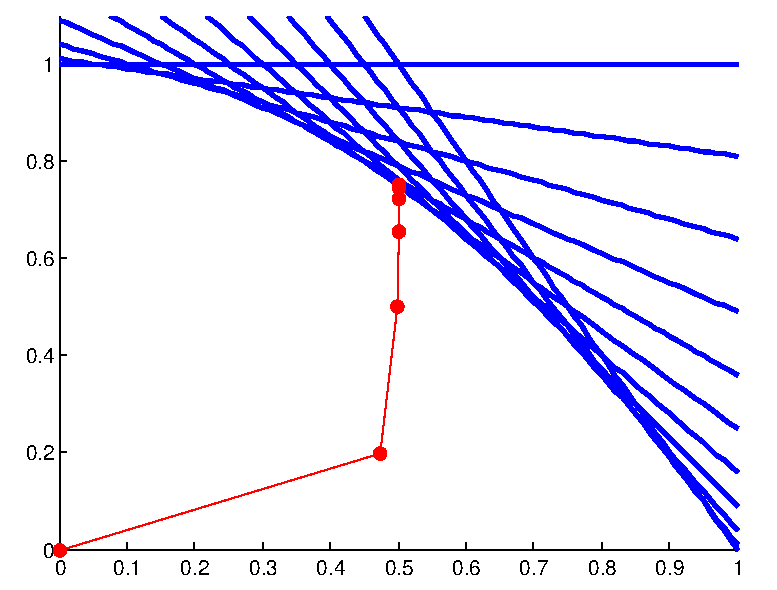
\includegraphics[width=0.7\textwidth]{images/lect12_cropped.pdf}
 \caption{Trajectory of long-step path-following in the $y_1-y_2$ plane.}\label{fig:fig1}
\end{figure}
It is instructive to play around with the parameter $\sigma$ and to try to determine the form of the central path in this example.

Another way to visualise the trajectory is to plot the pairs $x_is_i$ and $x_jy_j$ against each other.
Figure~\ref{fig:fig2} shows the trajectory of the above example in the $x_2s_2-x_5s_5$ plane. Note that the  central path, plotted in blue, is trivial in these coordinates, as it is defined by the property of the $x_is_i=\tau$ being equal.
\begin{figure}[h!]
\centering
 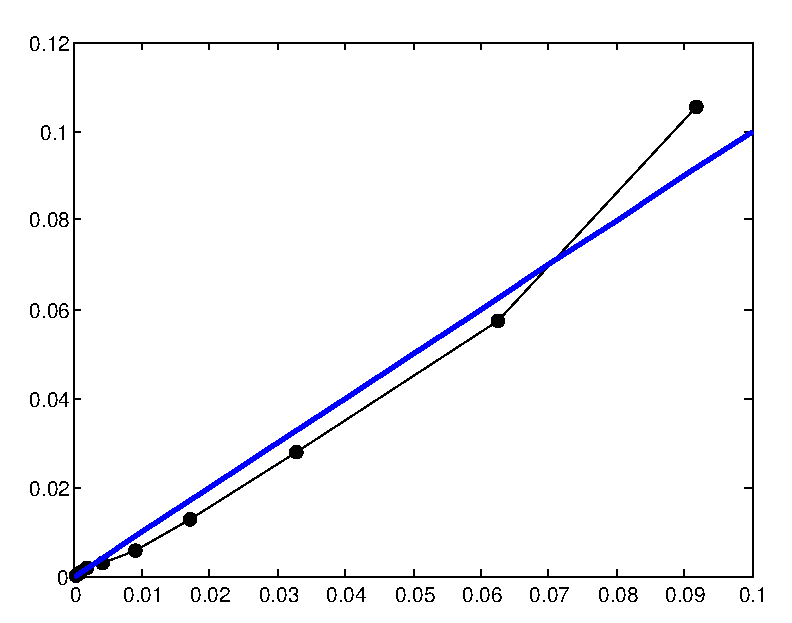
\includegraphics[width=0.7\textwidth]{images/lect12b_cropped.pdf}
 \caption{Trajectory and central path in $x_2s_2-x_5s_5$ coordinates.}\label{fig:fig2}
\end{figure}

\section{Analysis of Path-following}
In the analysis of the long-step path-following algorithm, it is enough to establish that the duality measure $\mu^{(k)}$ converges to $0$ as $k\to \infty$. The reason is that $\mu=0$ forces all the products $x_is_i=0$, and since by design the other constraints are satisfied, this means that the sequence of points converges to a solution. The first theorem tells us that the $\mu_k$ decrease as $k$ increases. An elementary proof is given in Theorem 14.3 in Nocedal and Wright. It depends crucially on the assumption that the iterates remain inside the neighbourhood $\mathcal{N}_{-\infty}(\gamma)$ of the central path.

\begin{theorem}
 Given parameters $\gamma$, $\sigma_{\mathrm{min}}$ and $\sigma_{\mathrm{max}}$, there is a constant $\delta>0$, independent of $d$, such that
 \begin{equation}\label{thm:1}
  \mu_{k+1}\leq \left(1-\frac{\delta}{d}\right) \mu_k.
 \end{equation}
\end{theorem}

The next theorem gives a bound on the number of iterations needed to reduce the duality measure beyond any given $\e$.

\begin{theorem}
 Let $\e>0$ and $\gamma\in (0,1)$. Let $(\vct{x}^{(0)},\vct{y}^{(0)},\vct{s}^{(0)})\in \mathcal{N}_{-\infty}(\gamma)$ be a starting point such that the duality measure satisfies $\mu^{(0)}\leq \e^{-\kappa}$ for some constant $\kappa$. Then there is an index $K=O(d\log (1/\e))$ such that for all $k>K$,
 \begin{equation*}
  \mu_k \leq \e.
 \end{equation*}
In particular, the long-step path-following algorithm converges.
\end{theorem}

\begin{proof}
Repeatedly applying~\eqref{thm:1}, we get
\begin{equation*}
 \mu_{k} \leq \left(1-\frac{\delta}{d}\right)^k \mu_0.
\end{equation*}
Taking logarithms on both sides,
 \begin{align*}
  \log \mu_{k}\leq k \log\left(1-\frac{\delta}{d}\right)+\log \mu_0 
  &\leq k \log\left(1-\frac{\delta}{d}\right)+\kappa \log\left(\frac{1}{\e}\right)\\
  &\leq k\frac{-\delta}{d}+\kappa\log\left(\frac{1}{\e}\right).
 \end{align*}
We have $\mu_k<\e$ if 
\begin{equation*}
 -k\frac{\delta}{d}+\kappa \left(\frac{1}{\e}\right) \leq \log \e,
\end{equation*}
of equivalently, if 
\begin{equation*}
 k\geq (1+\kappa)\frac{d}{\delta}\log\left(\frac{1}{\e}\right)=K.
\end{equation*}
This was to be shown.

\end{proof}



% %-----------------------------------------------------------------------
% % End of chap1.tex
% %-----------------------------------------------------------------------
